% CVPR 2022 Paper Template
% based on the CVPR template provided by Ming-Ming Cheng (https://github.com/MCG-NKU/CVPR_Template)
% modified and extended by Stefan Roth (stefan.roth@NOSPAMtu-darmstadt.de)

\documentclass[10pt,twocolumn,letterpaper]{article}

\usepackage[review]{cvpr}     
\usepackage{graphicx}
\usepackage{amsmath}
\usepackage{amssymb}
\usepackage{booktabs}


% It is strongly recommended to use hyperref, especially for the review version.
% hyperref with option pagebackref eases the reviewers' job.
% Please disable hyperref *only* if you encounter grave issues, e.g. with the
% file validation for the camera-ready version.
%
% If you comment hyperref and then uncomment it, you should delete
% ReviewTempalte.aux before re-running LaTeX.
% (Or just hit 'q' on the first LaTeX run, let it finish, and you
%  should be clear).
\usepackage[pagebackref,breaklinks,colorlinks]{hyperref}


% Support for easy cross-referencing
\usepackage[capitalize]{cleveref}
\crefname{section}{Sec.}{Secs.}
\Crefname{section}{Section}{Sections}
\Crefname{table}{Table}{Tables}
\crefname{table}{Tab.}{Tabs.}


%%%%%%%%% PAPER ID  - PLEASE UPDATE
\def\cvprPaperID{*****} % *** Enter the CVPR Paper ID here
\def\confName{CVPR}
\def\confYear{2022}


\begin{document}

%%%%%%%%% TITLE - PLEASE UPDATE
\title{COMP-6721 Project Proposal}

% \author{First Author\\
% Institution1\\
% Institution1 address\\
% {\tt\small firstauthor@i1.org}
% % For a paper whose authors are all at the same institution,
% % omit the following lines up until the closing ``}''.
% % Additional authors and addresses can be added with ``\and'',
% % just like the second author.
% % To save space, use either the email address or home page, not both
% \and
% Second Author\\
% Institution2\\
% First line of institution2 address\\
% {\tt\small secondauthor@i2.org}
% }
\maketitle



%%%%%%%%% BODY TEXT
\section{Problem Statement and Application}
\label{sec:problemstatement}
Recently, IoT nodes are becoming more common in cities as they become technologically advanced. Most of these nodes are low-power embedded systems and lack sufficient computing power. These nodes of the IoT use low power-wireless communication methods to communicate with each other and servers. One of the applications of these nodes is object detection, which can be used for security purposes and self-driving cars. There are many image classification models that can be applied on these nodes to classify objects. However, these models require high computing power to be implemented, which makes them unsuitable for IoT devices with low processing power. To resolve this problem, IoT nodes can send their images to a server with sufficient computing power to perform image classification and object detection. Therefore, the nodes should send the image data through a low-power wireless communication protocol such as Zigbee and LoraWAN. Since the data transfer rate of low-power wireless communication is low, IoT nodes must compress the images before transmitting them. The encoded image is transmitted through a noisy communication channel and at the decoder, the image is decoded. Considering that the communication medium has noise, some noise is added to the encoded image, which makes the decoder unable to recover the original image well. As a result, image classifiers cannot identify and classify images well. Inspired by article\cite{Alpher07}, we are going to simulate a model of a wireless communication system and develop an encoder and decoder using Pytorch. Figure 1 illustrates the architecture of this system. 
\begin{figure}[h]
    \centering
    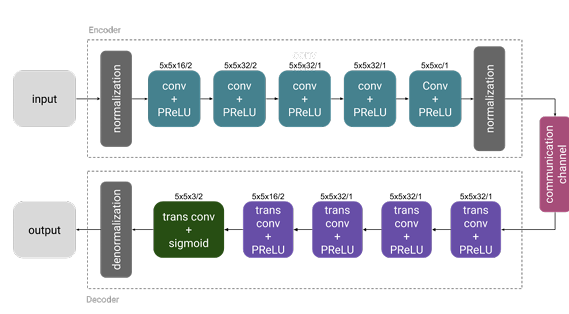
\includegraphics[scale=0.5]{ae.png}
    \caption{Proposed wireless image transmission system in \cite{Alpher07}}
\end{figure}
As it is clear from Figure 1, in the proposed system, first the image is encoded using neural network convolution, and then the encoded image is normalized by modularization to match the channel capacity, and then enters the noisy channel. This channel is considered AWGN channel by the authors of the article. In the AWGN channel, the Gaussian noise is added to the data. On the decoder side, the decoder gets noisy data from the channel and decodes the original image. Although using the deep autoencoder approach in this paper improves the quality of the decoded image in comparison with a classic approach such as JPEG image encoding, image recognition may still be difficult for image classifiers, especially when the channel has a lot of noise. Our goal in this project is to provide a classifier in the receiver section, to be able to classify the images sent by the sender with the highest possible accuracy. We plan to jointly train the image classifier model with the wireless communication model. 
We expect that since the image classification model is trained with channel noise, it will perform better than the model that is not trained with model noise.
\section{Dataset Selection} 
\label{sec:dataset}
Our selected data for this project is the CIFAR-100 dataset\cite{Alpher08}. A total of 60000 32x32 color images are included in the CIFAR-100 dataset, with 600 images per class. This dataset is downloadable from \cite{Alpher09}. The figure2 is an example of CIFAR-100 images.
\begin{figure}[h]
    \centering
   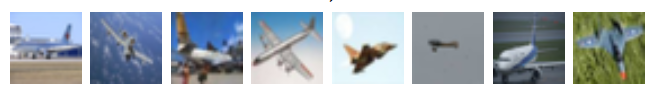
\includegraphics[scale=0.55]{cifar100.png}
    \caption{CIFAR-100 images \cite{Alpher08}}
\end{figure}
\section{Possible Methodology}
\label{sec:possiblemethodology}
In this project, we are going to train our model with three different structures. In the first model, we train the image classifiers independently of the wireless communication model to measure its maximum accuracy and then use it to classify the output images of the wireless communication network which have noise to see what effect it has on its accuracy. In the second model, we are going to train classifiers and the wireless communication model jointly. In this model, we are going to decode the image on the receiver side and then classify it using our image classifiers. In fact, we will add classifiers on the receiver side and after the decoder module. In the third model, instead of decoding the image on the receiver side, we intend to directly classify the encoded image containing noise obtained from the noisy channel. In this method, our classifiers are trained in such a way that instead of being able to classify the raw image, it classifies the encoded image. To evaluate the performance of the classifier, we use metrics such as Accuracy, F1-score, and Confusion matrix. In this project, the noisy channel is considered as an AWGN channel, as in article \cite{Alpher07}. We use the SNR metric to calculate the noise factor in a channel and noise factor affects the intensity of Gaussian noise that is added to the encoded image in a noisy channel. Finally, we test our models at various SNRs and compare their performance to see which model performs best.
%%%%%%%%% REFERENCES
{\small
\bibliographystyle{ieee_fullname}
\bibliography{egbib}
}

\end{document}

